
While analyzing the polarization images, we identified a faint background source at \bfiverob and \bsevenNS. In the \bfive data used for the majority of the analysis (\texttt{robust = -1}), the background source is not detected. Figure \ref{fig: GalaxyContamination_Both_Bands} shows the \SI images at \bfive and \bsevenNS, where the background source is visible slightly offset to the right of the disk, at the same position at both wavelengths. The source is not detected at \bfour and \bsixNS, likely due to differences in sensitivity. 


% ---------------------------------------------------------

% \begin{figure*}[h]
%   \centering
%   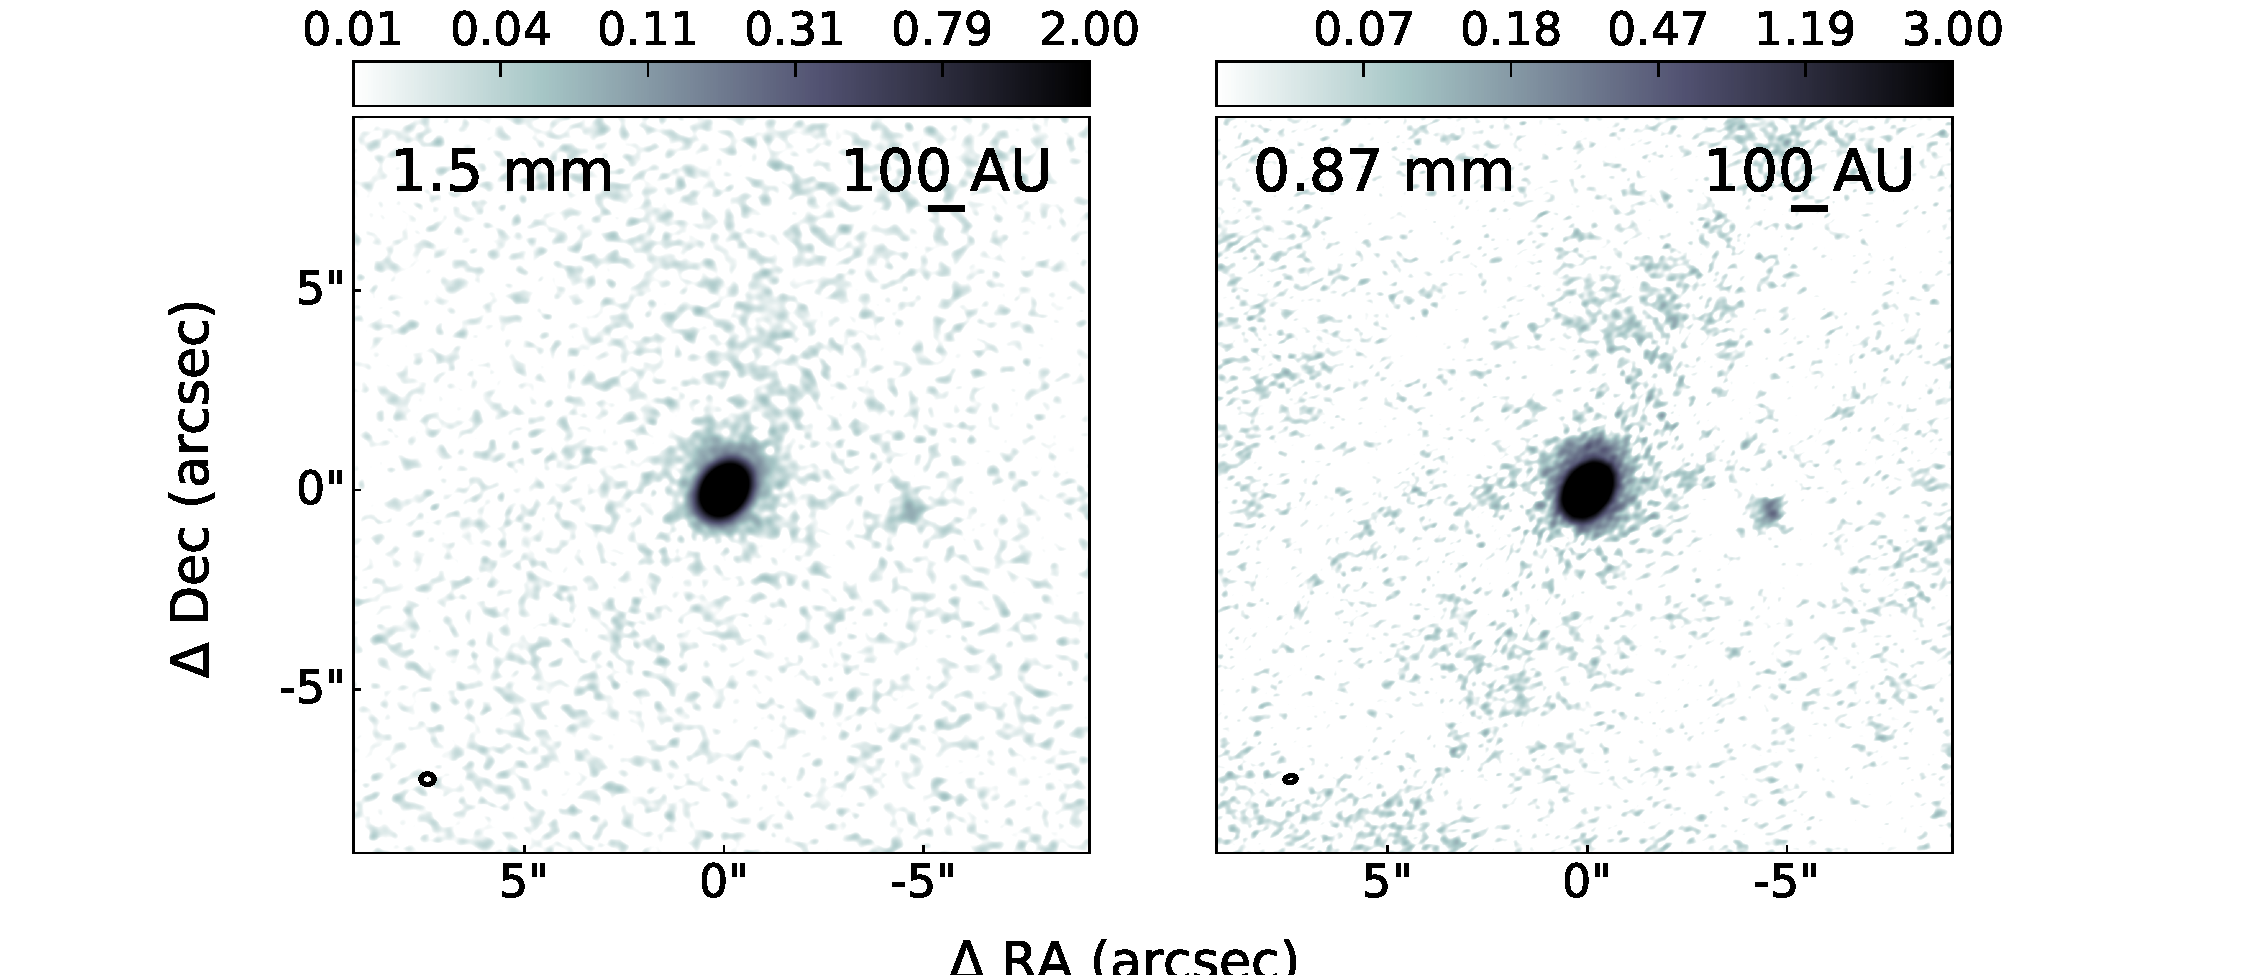
\includegraphics[width=1.1\textwidth]{../IMAGES/WRITEUP/GalaxyContamination/StokesI_BothBands.pdf}
%   \caption{Stokes I images of Band 5 (left) and Band 7 (right) to show the background source to the right of the disk. Note that the lowest and highest Stokes I values are cut off for visualization. Band 5 ranges: (-0.05710974, 79.41323) $\ra$ (0.006, 2) and Band 7 ranges: (-0.14653777, 175.78313) $\ra$ (0.02, 3), all values in mJy and were chosen by eye.  \question{Should I add a marker to show it's the same location? A circle?}}
%   \label{fig: GC_StokesI_BothBands}
% \end{figure*}




% \begin{figure*}[h]
%   \centering
%   % First figure
%   \begin{minipage}{0.48\textwidth}
%     \centering
%     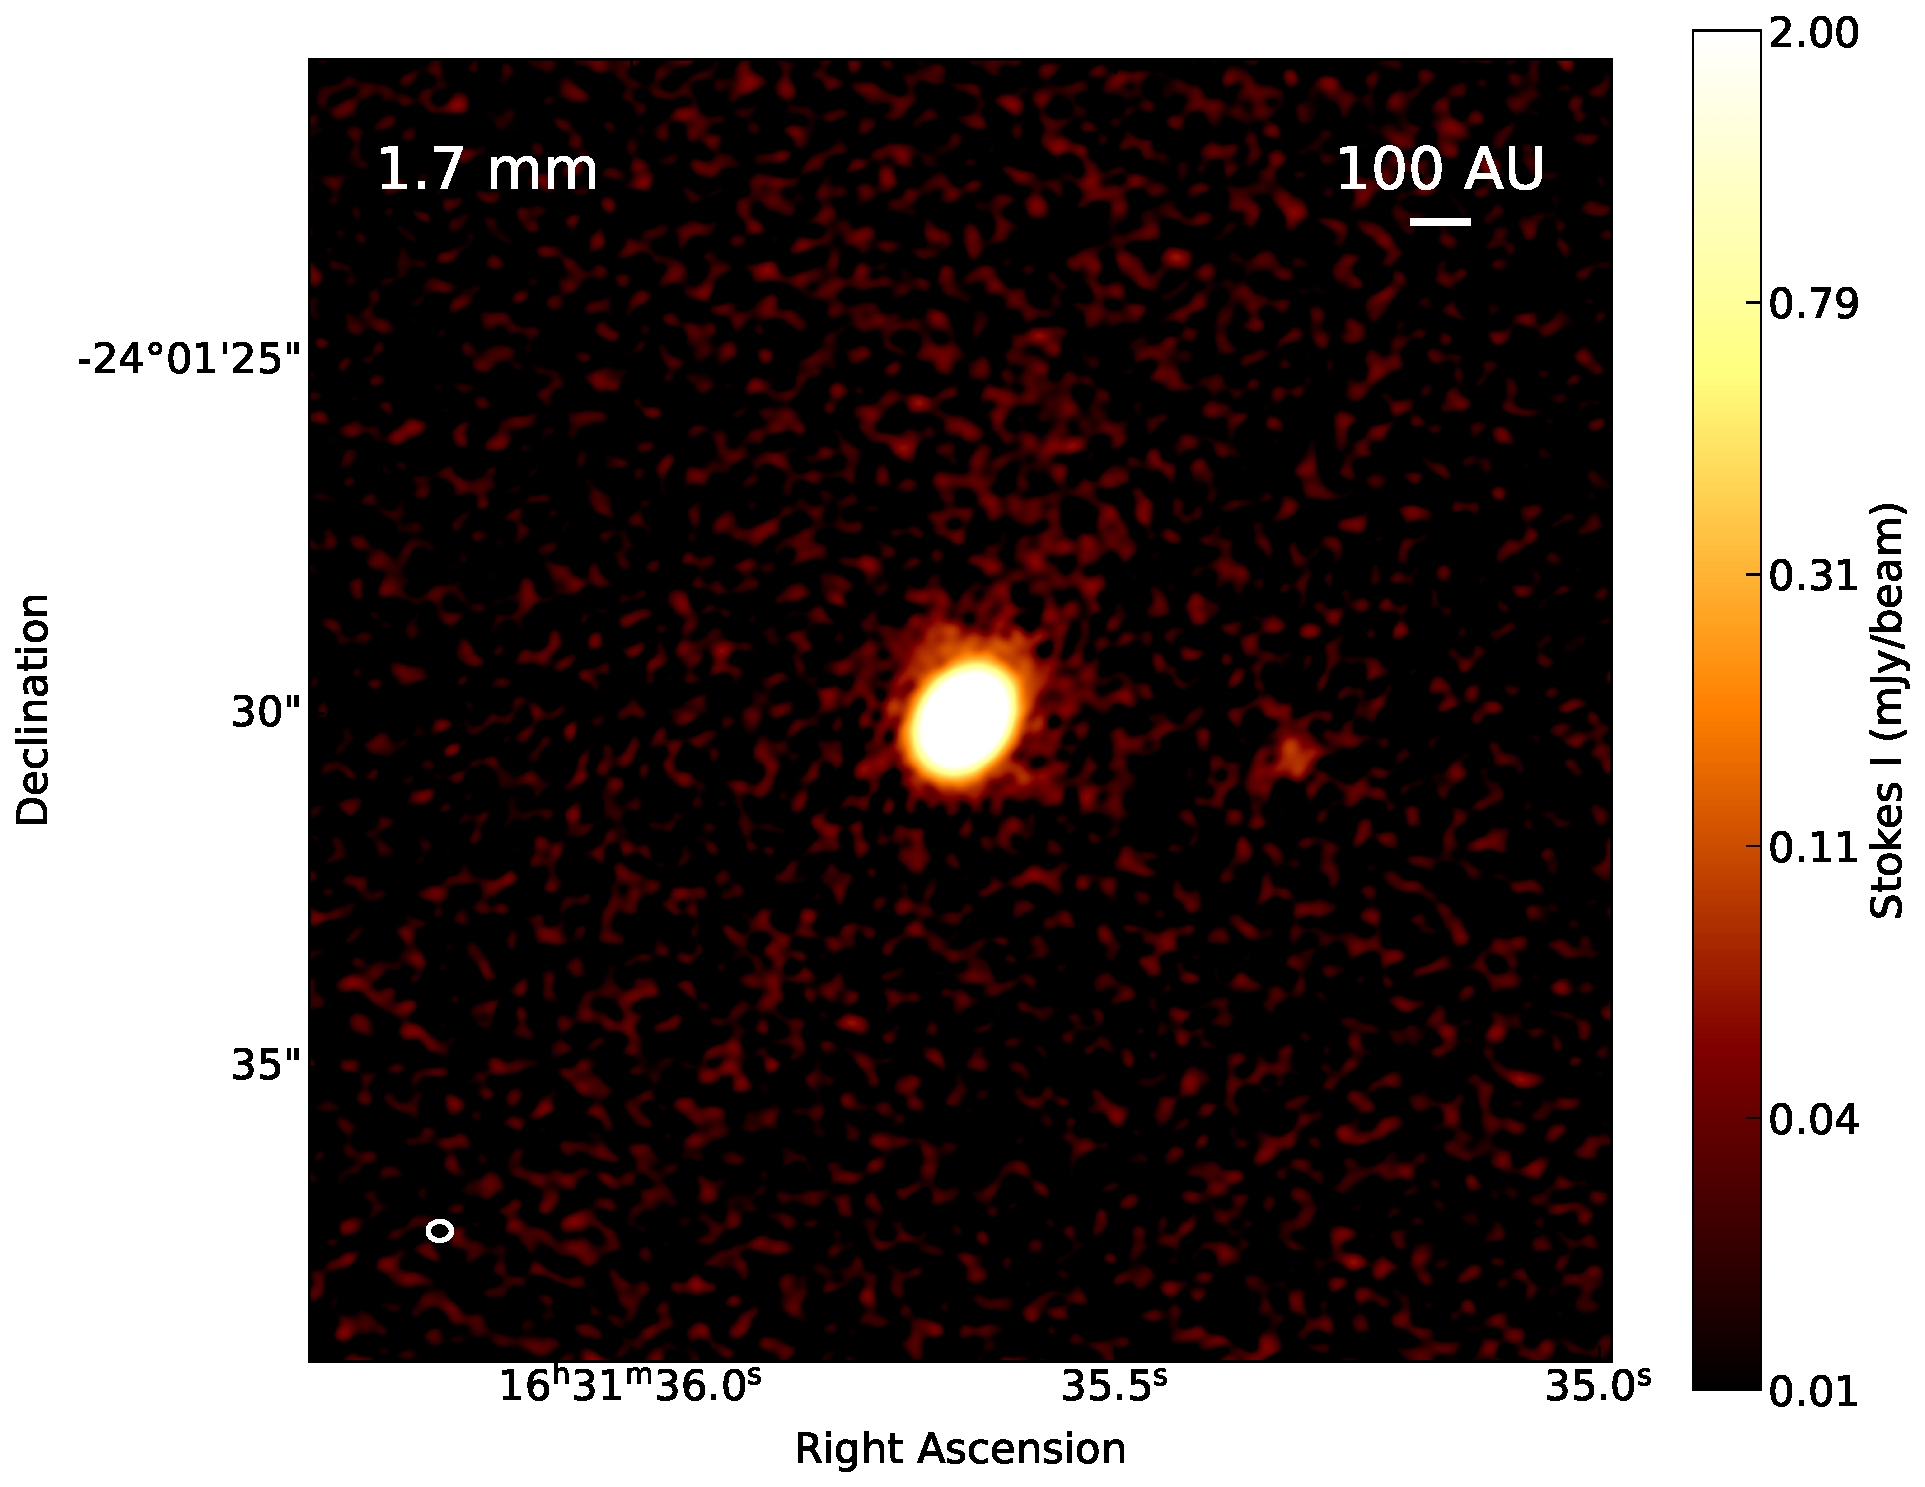
\includegraphics[width=\linewidth]{WRITEUP_AND_IMAGES/IMAGES/WRITEUP/GalaxyContamination/StokesI_BAND5.pdf}
%     \caption{Galaxy Contamination of Band 5. Note that Stokes I is cut off for visualization.}
%     \label{fig: GC_POLI_Band5}
%   \end{minipage}%
%   \hfill
%   % Second figure
%   \begin{minipage}{0.48\textwidth}
%     \centering
%     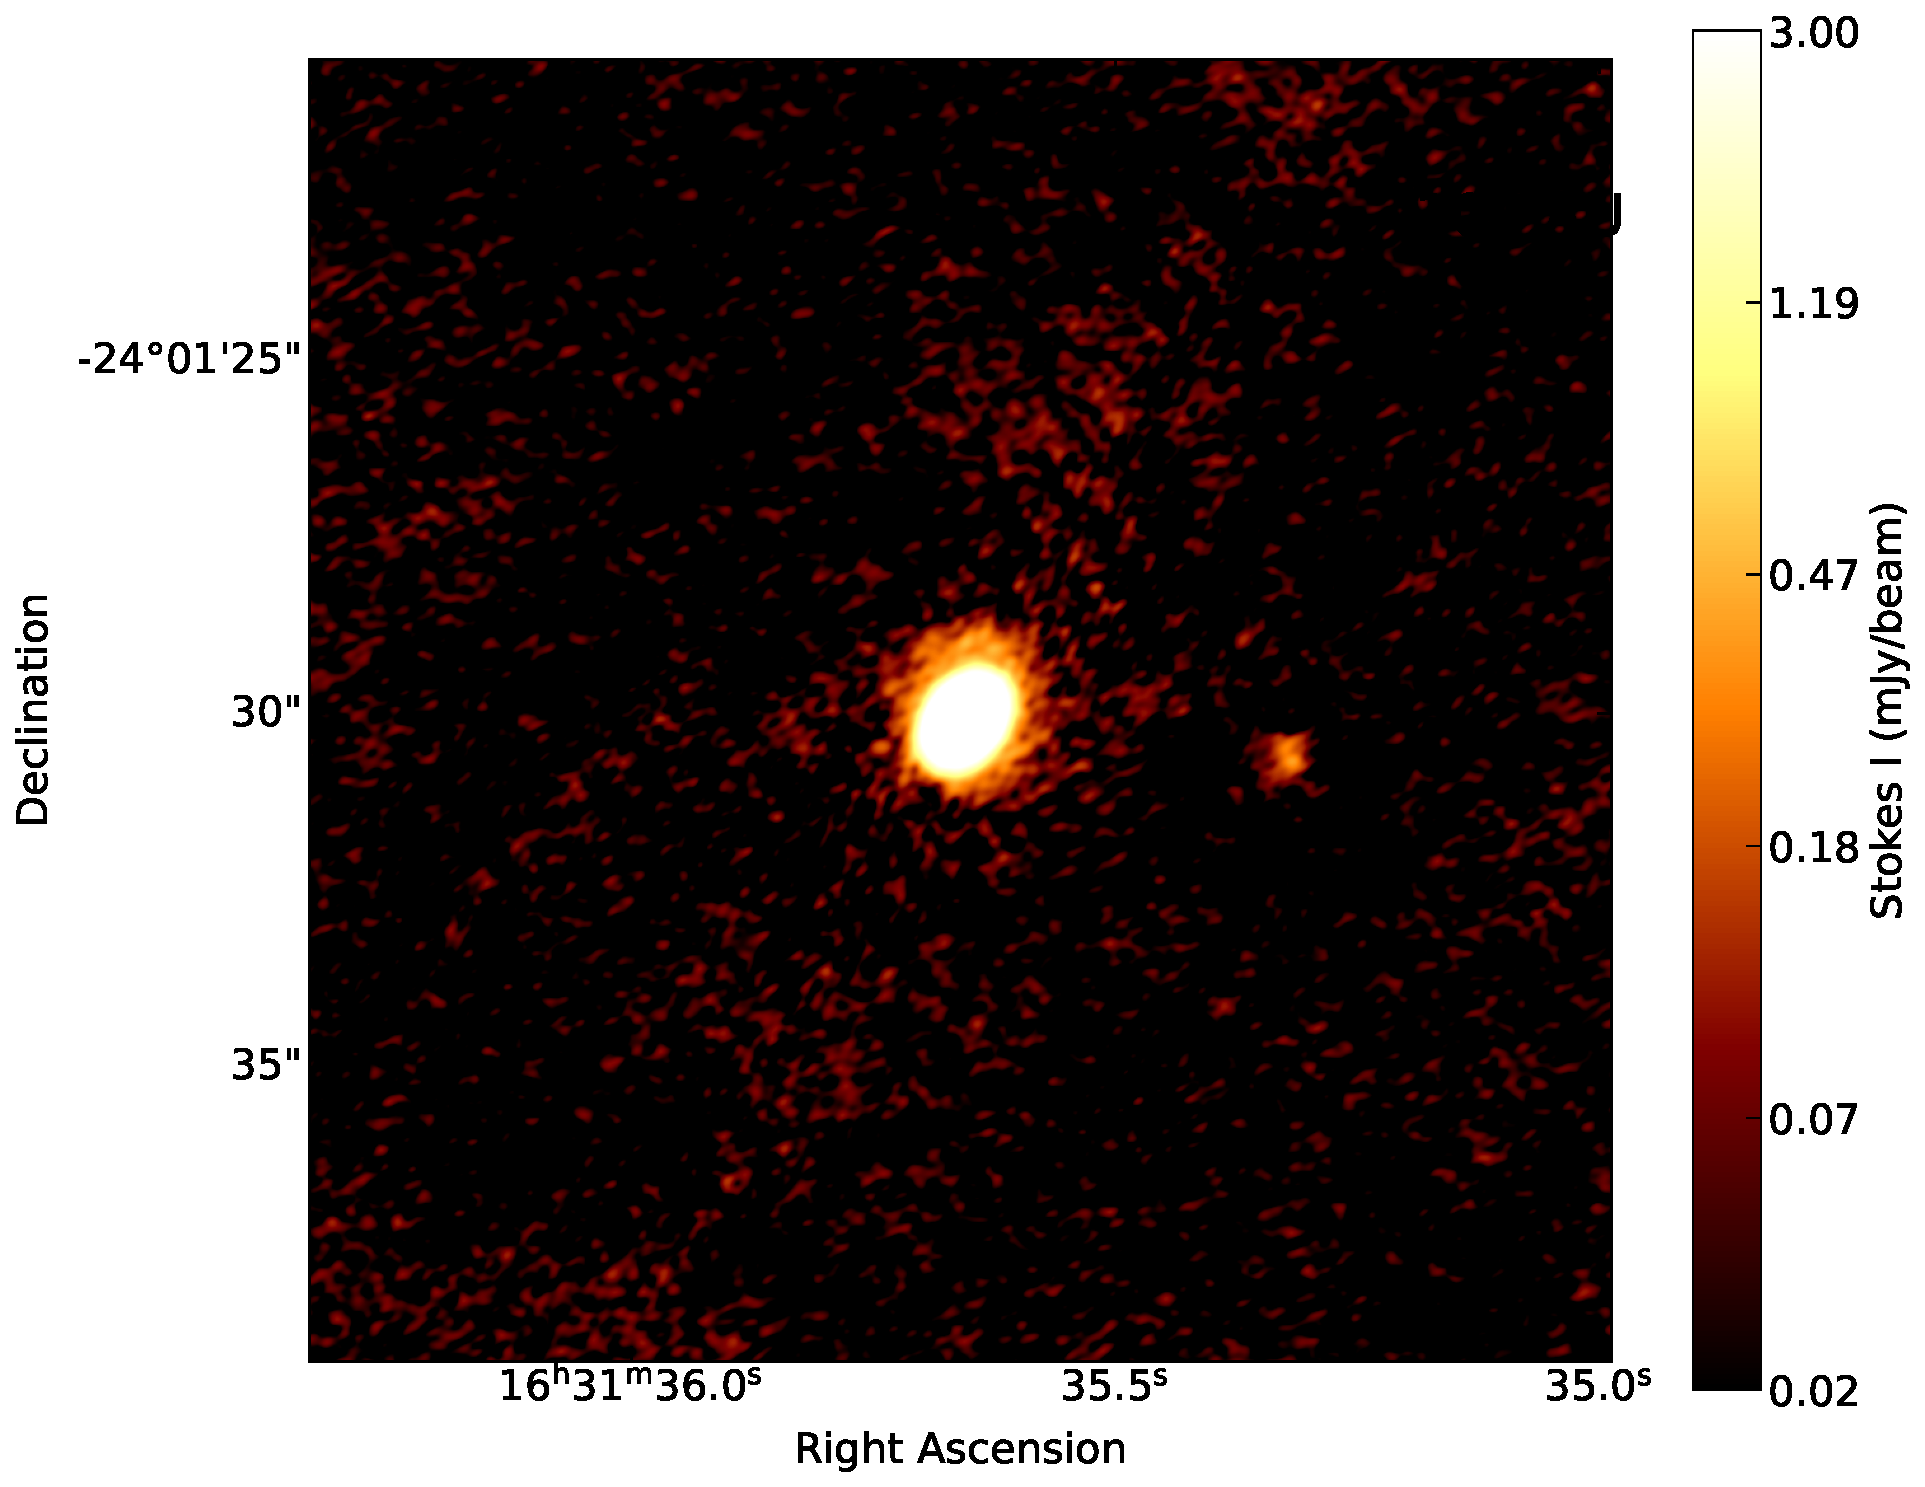
\includegraphics[width=\linewidth]{WRITEUP_AND_IMAGES/IMAGES/WRITEUP/GalaxyContamination/StokesI_BAND7.pdf}
%     \caption{Same as Figure \ref{fig: GC_POLI_Band5}, but for Band 7. Note that Stokes I is cut off for visualization.}
%     \label{fig: GC_POLI_Band7}
%   \end{minipage}
% \end{figure*}



\begin{figure*}[htbp]
  \centering
  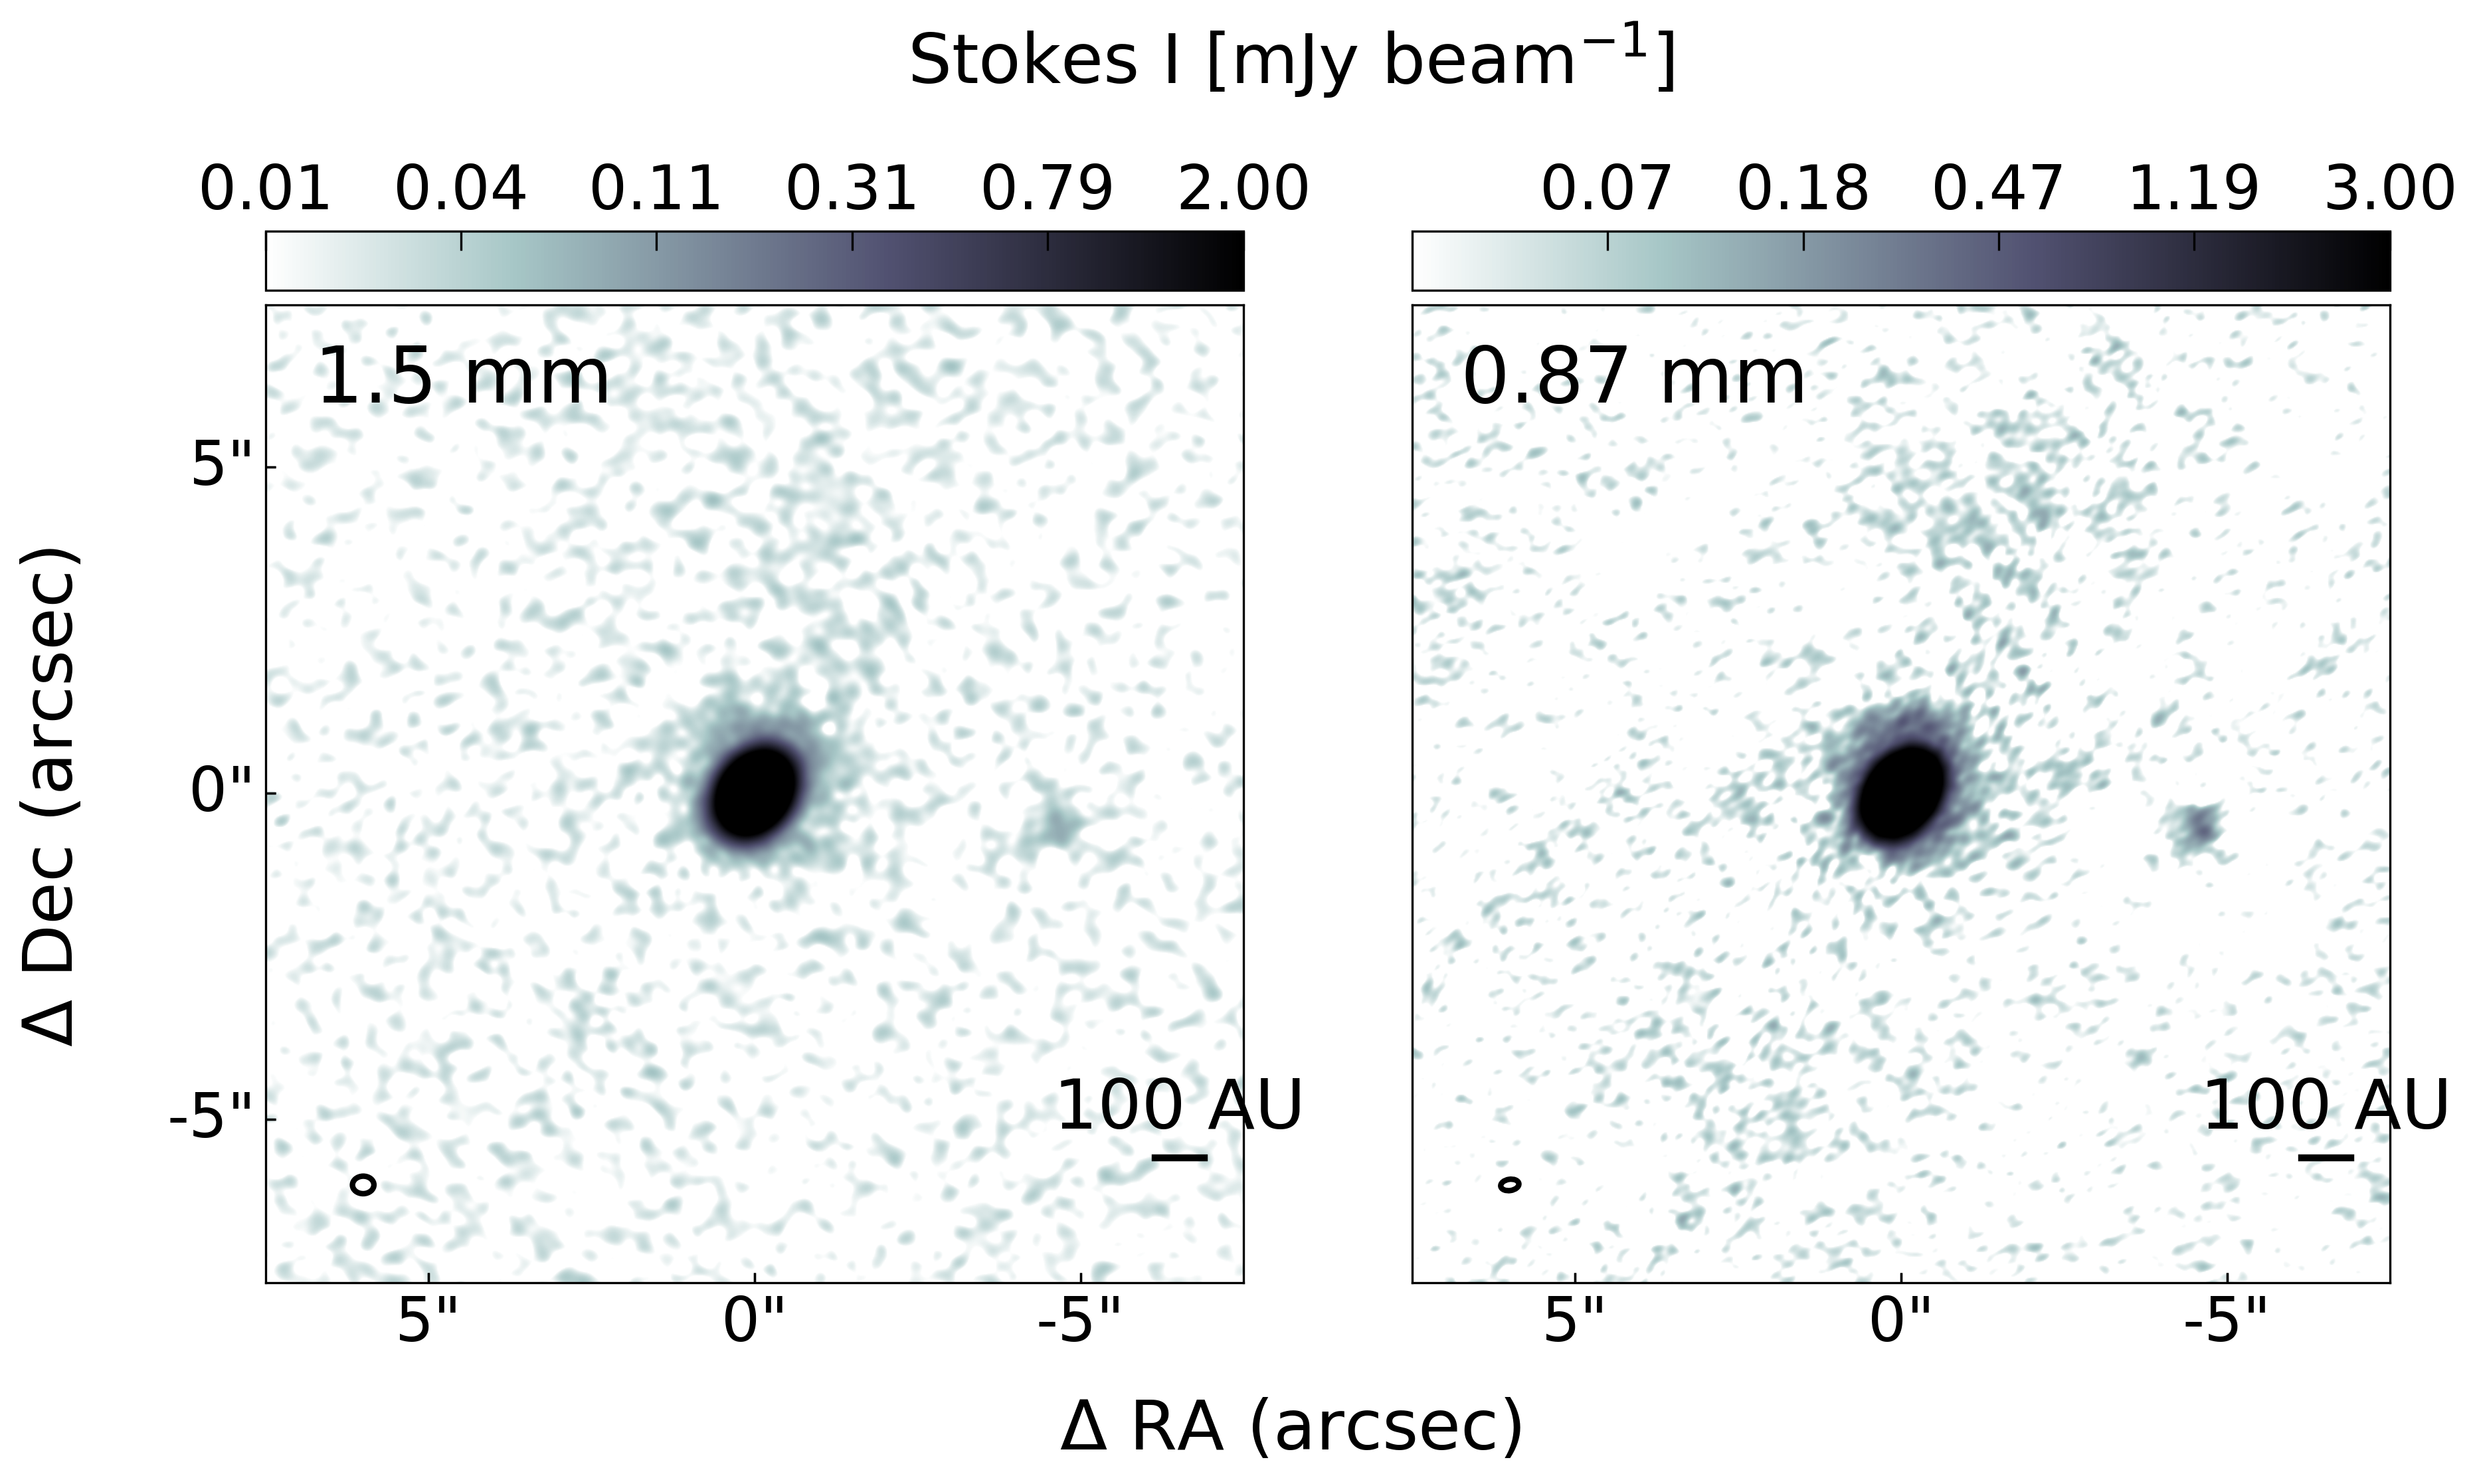
\includegraphics[width=0.99\textwidth]{WRITEUP_AND_IMAGES/IMAGES/WRITEUP/GalaxyContamination/StokesI_BothBands.png}
  \caption{\SI images at (left) \bfive (\texttt{robust = 0.5}) and (right) \bsevenNS, showing the detected background source. \code{AU to au}}
  \label{fig: GalaxyContamination_Both_Bands}
\end{figure*}


There are no known sources at the position of this object, suggesting that it could be a background galaxy. We estimated the probability that the source is a background galaxy following the method from \cite{sadavoy_dust_2019}. This method has also been used in other studies to estimate the number counts of background galaxies \citep{Carniani, Fujimoto}. Number counts are not well constrained at \bfiveNS, so the analysis is done only at \bsevenNS.


The galaxy number counts are described using the  Schechter function, which calculates $dN/dS$, the number of galaxies at a given flux per unit area on the sky.  The equation is given by:

\begin{equation}
\frac{dN}{dS}= N_0 \left(\frac{S}{S_0}\right)^\alpha \exp \left(- \frac{S}{S_0}\right),
\label{eq: GC_Schecter}
\end{equation}

\noindent where $N_0$ is the normalization factor, $S_0$ is the flux density at the turnover in mJy, $S$ is the intensity of the source, and $\alpha$ is the slope of the distribution \citep{Schechter}. The \bseven galaxy number counts used in the analysis were based on \cite{GC_Number_Counts}, and the background source has an intensity of $\sim$ 0.40 mJy. Substituting these values into Equation \ref{eq: GC_Schecter} gives:
\begin{equation}
\left.\frac{dN}{dS}\right|_{0.87 \text{ mm}}
= 923\left(\frac{0.40}{3.9}\right)^{-1.7}
\exp\left(-\frac{0.40}{3.9}\right).
\label{eq: GC_Schecter_B7}
\end{equation}







To account for the changes in sensitivity across the field of view, three detection thresholds were chosen: $5\sigma(r)$, $9\sigma(r)$, and $20\sigma(r)$. Here, $\sigma(r)$ is the noise as a function of the distance from the phase centre, increasing as sensitivity decreases as you move further from the phase centre. The noise at the phase centre was chosen to be $\sigma$ = 0.035 mJy, based on the \SI uncertainty at this wavelength reported in Table \ref{tab: source_info}. The noise as a function of radius is represented by the equation:
\begin{equation}
    \sigma(r) = \frac{0.035 \text{ mJy}}{\text{PB}(r)},
\end{equation}
\noindent where PB$(r)$ is the primary beam map.



The probability of detecting a background galaxy was calculated at concentric annuli with a radius of 0.25 arcsec. For each detection threshold, $dN/dS$ was integrated to determine the expected number of galaxies per unit area. This value was multiplied by the area of each annulus to determine the expected number of galaxies in each annulus, and converted to a probability using Poisson statistics:
\begin{equation}
    \text{Probability} = 100*(1 - \exp(-N_\text{expected})).
\end{equation}


\noindent Both the probability within each annulus and the cumulative probability as a function of radius are shown in Figure \ref{fig: GalaxyContamination_Prob_B7}. 



The background source is located $\sim$ 4.75 arcsec from the centre of the disk. At this radius, the cumulative probabilities for sources with thresholds of $5\sigma(r)$, $9\sigma(r)$, and $20\sigma(r)$ are 58.49\%, 39.89\%, and 19.55\%,  respectively. The source has a \SNR of approximately 9.44. Therefore, the $9\sigma(r)$ result is the best estimate of the probability. The probability of 19.55\% suggests that it is likely that the detected source is a background galaxy. Although the probability is non-negligible, the background source does not affect the main science goals of the project, as it is not a part of IRS 63, and it was not detected in the \bfive (\texttt{robust = -1}) data used for the majority of the analysis.







\begin{figure}[htbp]
  \centering
  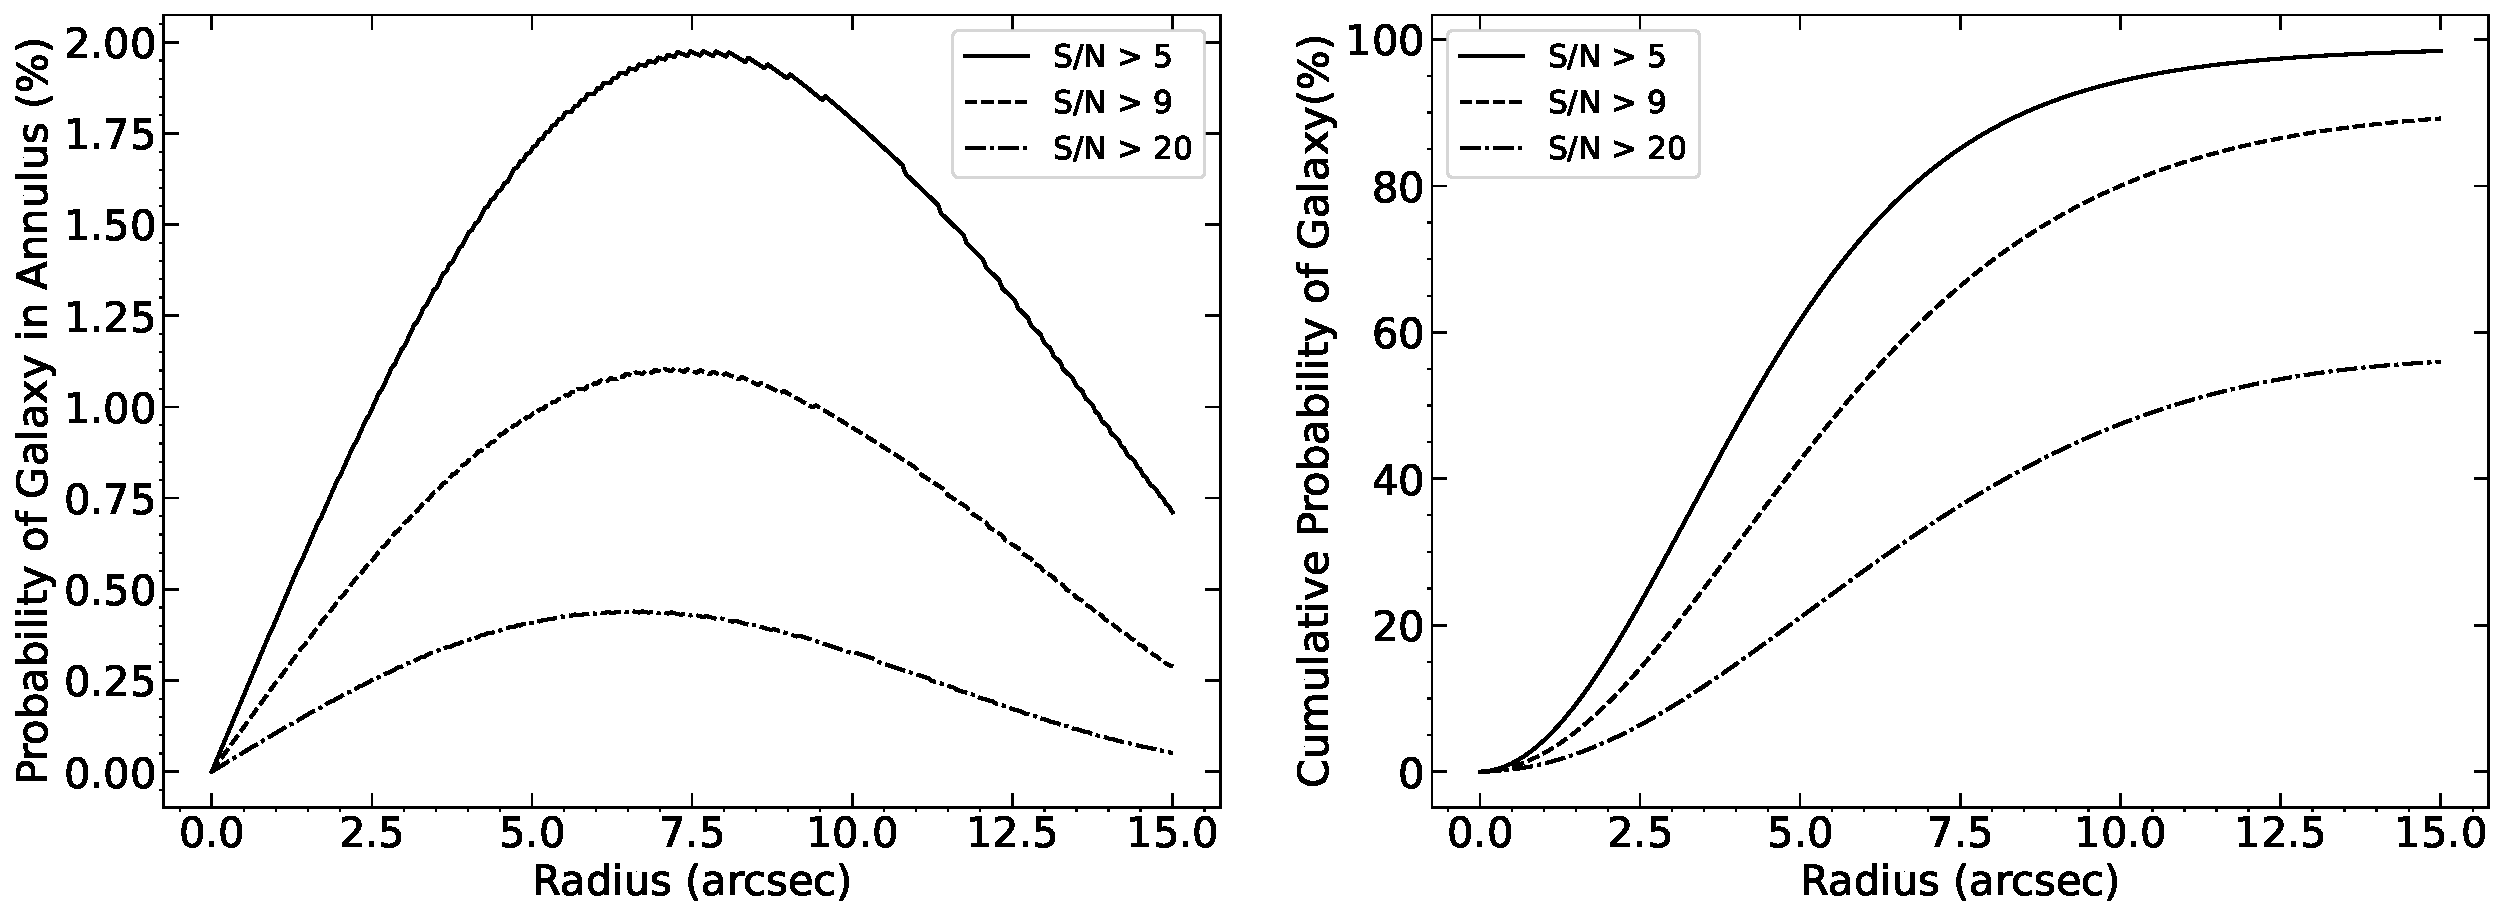
\includegraphics[width=0.99\textwidth]{WRITEUP_AND_IMAGES/IMAGES/WRITEUP/GalaxyContamination/Probabilities_Band7.pdf}
  \caption{Probability of detecting a background galaxy within an annulus (left) and cumulative probability within a given radius (right) at \bsevenNS, for detection thresholds of 5$\sigma$, 9$\sigma$ and 20$\sigma$}
  \label{fig: GalaxyContamination_Prob_B7}
\end{figure}







